\documentclass{beamer}
\mode<presentation> {

% The Beamer class comes with a number of default slide themes
% which change the colors and layouts of slides. Below this is a list
% of all the themes, uncomment each in turn to see what they look like.
\usepackage{graphicx}
\usepackage{svg}
\usepackage{xspace}
%\usetheme{default}
%\usetheme{AnnArbor}
%\usetheme{Antibes}
%\usetheme{Bergen}
%\usetheme{Berkeley}
%\usetheme{Berlin}
%\usetheme{Boadilla}
%\usetheme{CambridgeUS}
%\usetheme{Copenhagen}
%\usetheme{Darmstadt}
%\usetheme{Dresden}
%\usetheme{Frankfurt}
%\usetheme{Goettingen}
%\usetheme{Hannover}
%\usetheme{Ilmenau}
%\usetheme{JuanLesPins}
%\usetheme{Luebeck}
\usetheme{Madrid}
%\usetheme{Malmoe}
%\usetheme{Marburg}
%\usetheme{Montpellier}
%\usetheme{PaloAlto}
%\usetheme{Pittsburgh}
%\usetheme{Rochester}
%\usetheme{Singapore}
%\usetheme{Szeged}
%\usetheme{Warsaw}

% As well as themes, the Beamer class has a number of color themes
% for any slide theme. Uncomment each of these in turn to see how it
% changes the colors of your current slide theme.

%\usecolortheme{albatross}
%\usecolortheme{beaver}
%\usecolortheme{beetle}
%\usecolortheme{crane}
%\usecolortheme{dolphin}
%\usecolortheme{dove}
%\usecolortheme{fly}
%\usecolortheme{lily}
%\usecolortheme{orchid}
%\usecolortheme{rose}
%\usecolortheme{seagull}
%\usecolortheme{seahorse}
%\usecolortheme{whale}
%\usecolortheme{wolverine}

%\setbeamertemplate{footline} % To remove the footer line in all slides uncomment this line
%\setbeamertemplate{footline}[page number] % To replace the footer line in all slides with a simple slide count uncomment this line

%\setbeamertemplate{navigation symbols}{} % To remove the navigation symbols from the bottom of all slides uncomment this line
}

\usepackage{graphicx} % Allows including images
\usepackage{booktabs} % Allows the use of \toprule, \midrule and \bottomrule in tables

%----------------------------------------------------------------------------------------
%	TITLE PAGE
%----------------------------------------------------------------------------------------

\title[Short title]{MedicBot: A New Virtual Assistance for the Children with Auditory Processing Disorder } % The short title appears at the bottom of every slide, the full title is only on the title page

\author{Do Dung Vu \\ Supervisor: Prof. Sylvie Ratt\'e} % Your name

\institute[ETS] % Your institution as it will appear on the bottom of every slide, may be shorthand to save space
{
Département de génie logiciel et des TI \\ % Your institution for the title page
\medskip
\textit{do-dung.vu.1@ens.etsmtl.ca } % Your email address
}
\date{\today} % Date, can be changed to a custom date

\begin{document}

\begin{frame}
\titlepage % Print the title page as the first slide
\end{frame}

\begin{frame}
\frametitle{Overview} % Table of contents slide, comment this block out to remove it
\tableofcontents % Throughout your presentation, if you choose to use \section{} and \subsection{} commands, these will automatically be printed on this slide as an overview of your presentation
\end{frame}

%----------------------------------------------------------------------------------------
%	PRESENTATION SLIDES
%----------------------------------------------------------------------------------------

%------------------------------------------------
\section{Introduction} % Sections can be created in order to organize your presentation into discrete blocks, all sections and subsections are automatically printed in the table of contents as an overview of the talk
%------------------------------------------------

\subsection{} % A subsection can be created just before a set of slides with a common theme to further break down your presentation into chunks

\begin{frame}
\frametitle{Introduction}
\begin{columns}[T]
	
\begin{column}{.45\textwidth}
	\begin{figure}
		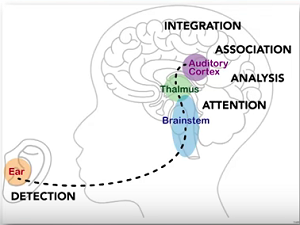
\includegraphics[width=50mm]{sound_processing_courtesy_asha.png}
		https://www.autismspeaks.org
	\end{figure}
\end{column}

\begin{column}{.6\textwidth}
	\begin{itemize}
		\item Auditory processing is defined as what we do with what we hear \footnote{Katz  \&  Tillery,  2004}
		\item Auditory Processing Disorder (APD) is a condition where someone has normal hearing, but the auditory system does not faithfully bring information to the brain \footnote{https://www.sac-oac.ca}
		\item \textbf{Approximate 2-4\% of school age children have APD} \footnote{http://www.ementalhealth.ca/}
		\item Autism and auditory processing disorders often overlap\footnote{https://www.autismspeaks.org}
	\end{itemize}
\end{column}
\end{columns}


\end{frame}
\begin{frame}
\frametitle{Challenging}
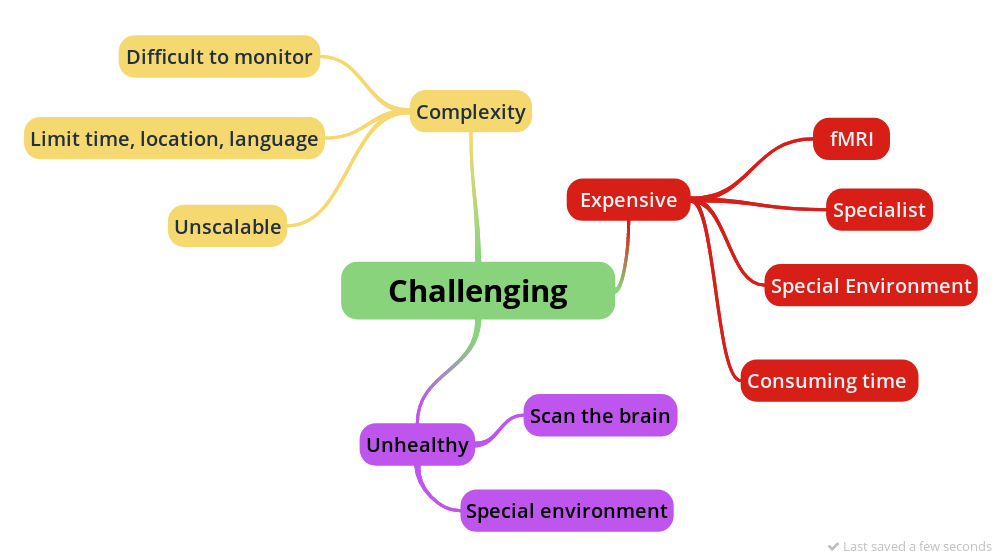
\includegraphics[width=120mm]{mind.jpg}

\end{frame}
\begin{frame}
\frametitle{Objectives}
Propose an AI model (virtual assitance) named \textcolor{blue}{\textbf{MedicBot}} to assit in diagnosing, monitoring, and training of the children with APD problem with low price, healthy, and convinent
\begin{columns}
	\begin{column}{.3\textwidth}
\begin{center}
		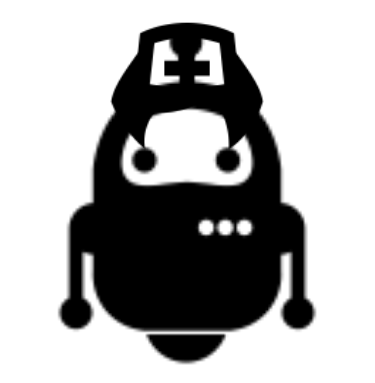
\includegraphics[width=30mm]{MedicBot.png}
	
\textbf{	MedicBot}
\end{center}

	\end{column}
\begin{column}{.7\textwidth}


\begin{itemize}
	\item Diagnose APD symptoms based on \textcolor{blue}{conversation} with the considered children
	\item Create a Training Therapy Model Assitance (adaptable)
	\item Build the Reinforcement Learining (RL) Model to monitor the progress of APD treatment
\end{itemize}



\end{column}
\end{columns}
\end{frame}
%------------------------------------------------
\section{Methodology } % Sections can be created in order to organize your presentation into discrete blocks, all sections and subsections are automatically printed in the table of contents as an overview of the talk
%------------------------------------------------
\subsection{} % A subsection can be created just before a set of slides with a common theme to further break down your presentation into chunks

\begin{frame}
	\frametitle{Methodology}
	\begin{itemize}
		\item Analysis  the  given  APD  symptoms  by  speech  	
		recognition  based  on  Deep  learning
		
		\item \color{gray} Analysis  the  given  APD  therapy  and  recommend  the
		
		treatment  to  the  APD  children.  Apply  a  natural  language
		
		processing  (NLP)  to  generate  sentences  and  exploit  Deep
		
		learning  to  understand  the  context  of  the  speech
		
		\item Monitoring  the  process  of  APD  treatment  by  using  speech  analysis  based  on  Deep
		
		learning
	\end{itemize}

\end{frame}


%------------------------------------------------
\section{Techniques } % Sections can be created in order to organize your presentation into discrete blocks, all sections and subsections are automatically printed in the table of contents as an overview of the talk
%------------------------------------------------
\begin{frame}
\frametitle{Implementation}
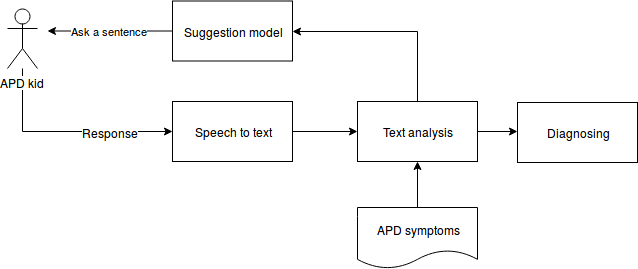
\includegraphics[width=120mm]{process.png}
\end{frame}

\begin{frame}
\frametitle{Techniques}
\textbf{Convert speech to text}
\begin{columns}[T]
		\begin{column}{.5\textwidth}
		
		\begin{itemize}
			
		\item	\textbf{Acoustic modeling} represents the relationship between linguistic units of speech and audio signals.
		\item	\textbf{Language modeling} matches sounds with word sequences to help distinguish between words that sound similar.
			
		\end{itemize}
		
	\end{column}
	\begin{column}{.5\textwidth}
				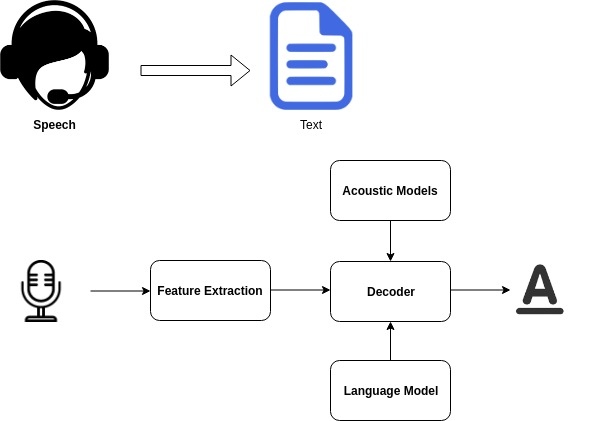
\includegraphics[width=65mm]{f1.jpg}
	\end{column}

\end{columns}
 {\small We evaluated the quality of output by using two factors:\footnote{https://pypi.org/project/SpeechRecognition/}\\

\textbf{Accuracy} and \textbf{Speed} }

\end{frame}

%------------------------------------------------


\begin{frame}
\frametitle{Techniques}
\textbf{Proposal for the objective 1 solution}
\begin{columns}[T]
	\begin{column}{.5\textwidth}
		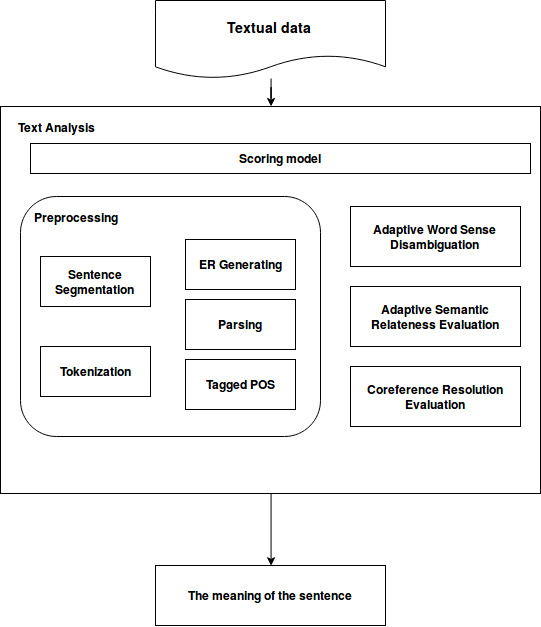
\includegraphics[width=55mm]{f21.jpg}
	\end{column}
	\begin{column}{.5\textwidth}
		
		\begin{itemize}
			\item Step 1: Get the raw text data from the user conversation
			\item Step 2: Process text go extract and compute the score of features 
			\item Step 3: Adapt word sense disambiguation
			\item Step 4: Evalue the semantic relateness and coreference resolution
			\item Step 5: Get the meaning of the sentence
		\end{itemize}
		
	\end{column}
\end{columns}

\end{frame}
\begin{frame}
\frametitle{Dataset}
\textbf{Open Dataset}
\begin{itemize}
{\scriptsize   	\item (NLVR) A Corpus of Natural Language for Visual Reasoning, 2017
	\item (MS MARCO) MS MARCO: A Human Generated MAchine Reading COmprehension Dataset, 2016
	\item (NewsQA) NewsQA: A Machine Comprehension Dataset, 2016 
	\item (SQuAD) SQuAD: 100,000+ Questions for Machine Comprehension of Text, 2016
\item 	(GraphQuestions) On Generating Characteristic-rich Question Sets for QA Evaluation, 2016 
\item 	(Story Cloze) A Corpus and Cloze Evaluation for Deeper Understanding of Commonsense Stories, 2016 
\item 	(Children's Book Test) The Goldilocks Principle: Reading Children's Books with Explicit Memory Representations, 2015 
\item 	(SimpleQuestions) Large-scale Simple Question Answering with Memory Networks, 2015
\item 	(WikiQA) WikiQA: A Challenge Dataset for Open-Domain Question Answering, 2015
\item 	(CNN-DailyMail) Teaching Machines to Read and Comprehend, 2015 
\item 	(QuizBowl) A Neural Network for Factoid Question Answering over Paragraphs, 2014 
\item 	(MCTest) MCTest: A Challenge Dataset for the \item Open-Domain Machine Comprehension of Text, 2013 
\item (QASent) What is the Jeopardy model? A quasisynchronous grammar for QA, 2007 }
\end{itemize}


\end{frame}
\begin{frame}
\frametitle{Dataset}
\begin{center}
	\textbf{Crawl dataset}\\
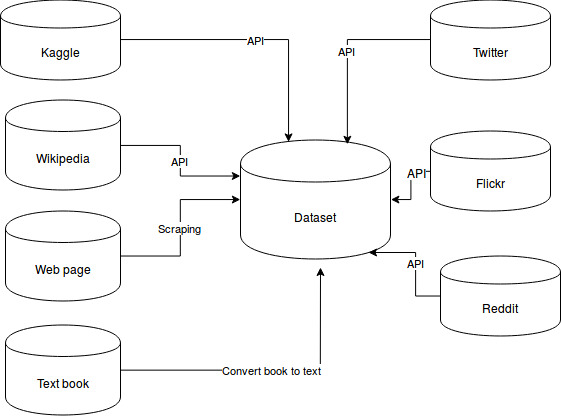
\includegraphics[width=80mm]{f9.jpg}
\end{center}
\end{frame}

\begin{frame}
\frametitle{Dataset}
\textbf{Paraphase database (PPDB)}
\begin{itemize}
	\item \textbf{PPDB}\footnote{http://paraphrase.org} is an automatically extracted database containing millions paraphrases in 16 different languages. 
	\item 
	The goal of PPBD is to improve language processing by making systems more robust to language variability and unseen words. 
	\item The entire PPDB resource is freely available under the Creative Commons Attribution 3.0 United States License.
	\item PPDB contains over 150 million paraphrase rules covering three paraphrase types lexical (single word), phrasal (multiword), and syntactic restructuring rules
\end{itemize}




\end{frame}


\begin{frame}
\frametitle{Chatbot}
\begin{columns}[T]
	\begin{column}{.5\textwidth}
		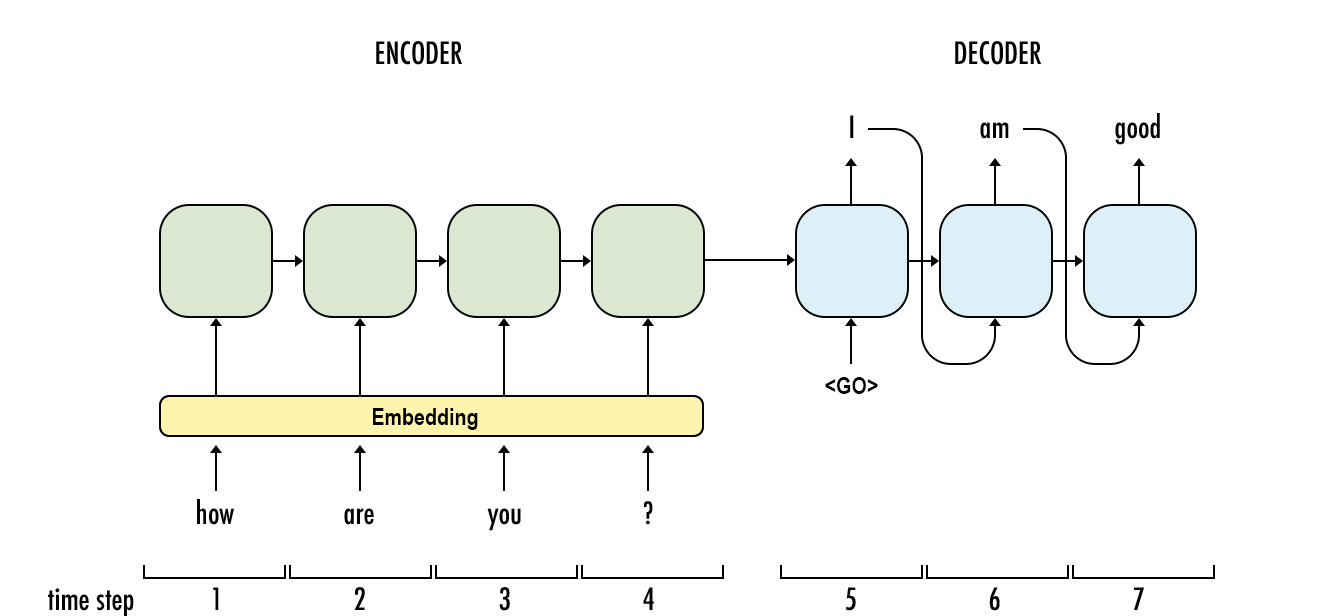
\includegraphics[width=65mm]{seq2seq.png}
		\begin{itemize}
		{\scriptsize 	\item $<PAD>$: During training, inputs in these batches all need to be the same width for the network to do its calculation. 
			\item $<EOS>$: It allows us to tell the decoder where a sentence ends, and it allows the decoder to indicate the same thing in its outputs as well.
		}
		\end{itemize}
	\end{column}
	\begin{column}{.5\textwidth}
		
		\begin{itemize}
{\scriptsize 
			\item $<UNK>$: If you’re training your model on real data, you’ll find you can vastly improve the resource efficiency of your model by ignoring words that don’t show up often enough in your vocabulary to warrant consideration. We replace those with $<UNK>$.
	
		\item $<GO>$: This is the input to the first time step of the decoder to let the decoder know when to start generating output.}
		\end{itemize}
		
	\end{column}
\end{columns}

\end{frame}


\begin{frame}
\frametitle{APD Symptoms}
\begin{table}[]
	\begin{tabular}{|l|llll}
		\cline{1-1}
		\textbf{Listening} &  &  &  &  \\ \cline{1-1}
	Has difficulty locating a sound source.	&  &  &  &  \\ \cline{1-1}
	Has difficulty hearing in noisy background. 	&  &  &  &  \\ \cline{1-1}
	Often asks for repetition or clarification 	&  &  &  &  \\ \cline{1-1}
	\textbf{Speaking}	&  &  &  &  \\ \cline{1-1}
Has difficulty answering open--ended questions	&  &  &  &  \\ \cline{1-1}
May speak in oversimplified short sentences with difficulties in syntax  	&  &  &  &  \\ \cline{1-1}
Mispronounced words, especially long words. 	&  &  &  &  \\ \cline{1-1}
\textbf{Phonological Awareness}	&  &  &  &  \\ \cline{1-1}
Has difficulty focusing during conversations	&  &  &  &  \\ \cline{1-1}
Forgets information that is easily heard 	&  &  &  &  \\ \cline{1-1}
	\end{tabular}
	\caption{A part of checklist for assessing whether the child with APD\footnote{https://kidshear.com.au}}
	\label{1}
\end{table}

\end{frame}

\begin{frame}
\frametitle{Process of creating model}
\begin{figure}
		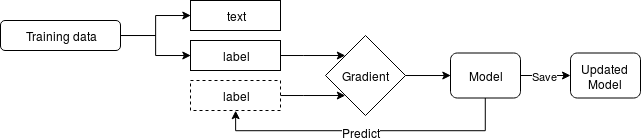
\includegraphics[width=.8\linewidth]{Spacy.png}
\end{figure}

\begin{itemize}
	\item  MedicBot's models are \textbf{statistical} and every "decision" she makes is a \textbf{prediction}
	\item This precision is based on the examples the model has seen during training
	\item We give the model feedback on its prediction in the form of an \textbf{error gradient} of the\textbf{ loss function} that calculates the difference between the training example and the expected output
\end{itemize}
\end{frame}


\begin{frame}
\frametitle{Techniques}
\textbf{Scoring model} 
\begin{columns}[T]
		\begin{column}{.5\textwidth}
			\begin{itemize}
				\item Create the features for the scoring model
				\item Compute the score for these ones
				\item Using the K-Mean Clustering algorithm to cluter the kid
				\item Apply the Elbow and K-validation algorithm to optimize the K-value of K-Mean Clustering algorithm
				\item Make the score table of considered kids
			\end{itemize}
		\end{column}
		\begin{column}{.7\textwidth}
			
			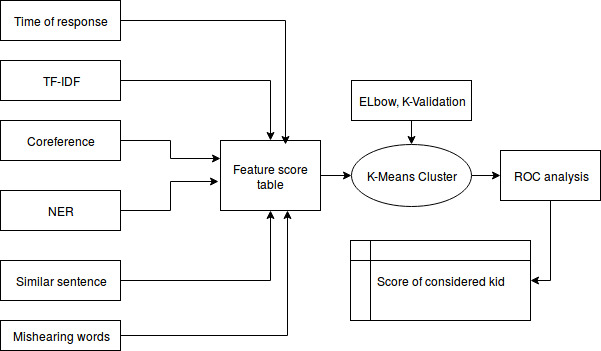
\includegraphics[width=65mm]{f6.jpg}
			
		\end{column}
	\end{columns}
	
\end{frame}

\begin{frame}
\frametitle{Techniques}
\textbf{Preprocessing} 
\begin{columns}[T]
	\begin{column}{.5\textwidth}
		\begin{itemize}
			\item Recognize the subject, verb, object in a given sentence
			\item Recoginze noun, adj, adv, preposition of a sentence
			\item Recognize the entities in a sentence
			\item Recognize the coreference of a sentence
		\end{itemize}
	\end{column}
	\begin{column}{.6\textwidth}
		
		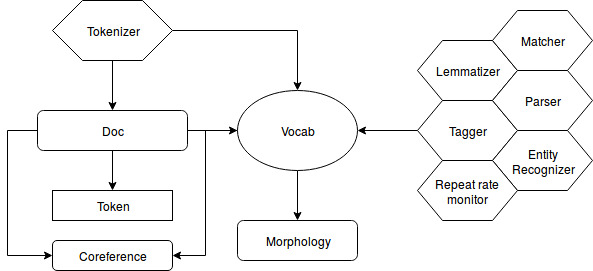
\includegraphics[width=65mm]{f5.jpg}
		
		
	\end{column}
\end{columns}



\begin{flushleft}
	$\rightarrow$ \textit{create the table of features }
\end{flushleft}

\end{frame}
\begin{frame}

\begin{table}[]
	\begin{tabular}{lllll}
		\cline{1-2}
		\multicolumn{1}{|l|}{time of response } & \multicolumn{1}{l|}{$\sum_{t=0}^{T}(t_i)$, $t_i$ the duration of one sentence} &  &   &  \\ \cline{1-2}
		\multicolumn{1}{|l|}{tf-idf(k,d,D)} & \multicolumn{1}{l|}{\begin{tabular}[c]{@{}l@{}}$tf(k,d)\times idf(k,D)$, $k$: term $k$\\ $d$: document $d$; and $d \in D$ \end{tabular} } &  &  &  \\ \cline{1-2}
		\multicolumn{1}{|l|}{coreference} & \multicolumn{1}{l|}{coreference resolution evaluation} &  &  &  \\ \cline{1-2}
		\multicolumn{1}{|l|}{ner} & \multicolumn{1}{l|}{name entity recognization}                                              &  &  &  \\ \cline{1-2}
			\multicolumn{1}{|l|}{similar sentence} & \multicolumn{1}{l|}{similarity evaluation}                                              &  &  &  \\ \cline{1-2}
				\multicolumn{1}{|l|}{mishearing word} & \multicolumn{1}{l|}{spelling and  grammar checking evaluation}                                              &  &  &  \\ \cline{1-2}
					\multicolumn{1}{|l|}{elbow algorithm} & \multicolumn{1}{l|}{choose a small value of k that still has a low SSE}                                              &  &  &  \\ \cline{1-2}
			\multicolumn{1}{|l|}{ROC analysis} & \multicolumn{1}{l|}{		 Receiver Operating Characteristic analysis}                                              &  &  &  \\ \cline{1-2}

	\end{tabular}
\end{table}


\end{frame}
\begin{frame}
\frametitle{Implementation}

\begin{table}[]
	\begin{tabular}{|l|l|}
		\hline
		\textbf{}                                           Requirements              & Content                                   \\ \hline
		\textbf{Python}                                                         & \begin{tabular}[c]{@{}l@{}} 2.6, 2.7, or 3.3+ \end{tabular} \\ \hline
		\textbf{PocketSphinx}                                              & \begin{tabular}[c]{@{}l@{}} large vocabulary speaker independent \\recognition system\end{tabular} \\ \hline
		\begin{tabular}[c]{@{}l@{}}\textbf{PyAudio}\end{tabular} & \begin{tabular}[c]{@{}l@{}} 0.2.11+ (required only if you need to\\ use microphone input, Microphone)\end{tabular} \\ \hline
		
		\textbf{SpeechRecognition}                                                         & \begin{tabular}[c]{@{}l@{}} a process in which a computer or device record\\ the speech of humans and convert it into text  \end{tabular} \\ \hline
		\textbf{Google API Client}                                                         & \begin{tabular}[c]{@{}l@{}} use the Google Cloud Speech API \end{tabular} \\ \hline
		\textbf{FLAC encoder}                                                         & \begin{tabular}[c]{@{}l@{}}if the system is not x86-based \\Windows/Linux/OS X \end{tabular} \\ \hline
	\end{tabular}
	\caption{Requirements of environment}
	\label{tab:setup}
\end{table}
\end{frame}
\begin{frame}
\frametitle{Implementation}
\begin{table}[]
	\begin{tabular}{|l|l|}
		\hline
		\textbf{}                                           Requirements              & Content                                   \\ \hline
		\textbf{SpaCy}                                                         & \begin{tabular}[c]{@{}l@{}} Industrial-Strength NLP \end{tabular} \\ \hline
		\textbf{NeuralCoref}                                              & \begin{tabular}[c]{@{}l@{}} Coreference Resolution in spaCy with Neural Netwo-\\rks \end{tabular} \\ \hline
		\begin{tabular}[c]{@{}l@{}}\textbf{NLTK}\end{tabular} &  \begin{tabular}[c]{@{}l@{}}Natural Language toolkit\end{tabular} \\ \hline
		
		\begin{tabular}[c]{@{}l@{}}\textbf{Scikit-learn} \\\textbf{Tensorflow} \\\textbf{Pytorch}   \end{tabular}                                                     & \begin{tabular}[c]{@{}l@{}} Machine learning library  \end{tabular} \\ \hline
		\textbf{ELMo}                                                         & \begin{tabular}[c]{@{}l@{}} Embeddings from Language Models \end{tabular} \\ \hline
	
	\end{tabular}
	\caption{Requirements of environment}
	\label{tab:setup}
\end{table}
\end{frame}
%\begin{frame}
%\frametitle{Coreference resolution evaluation}
%\begin{figure}
%	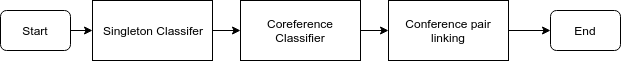
\includegraphics[width=.9\linewidth]{Coreference.png}
%\end{figure}
%\begin{itemize}
%	\item \textbf{Singleton classifier}: This classifier 
%	considers  five  representations  which  are  word,  dependency,  
%	string,  numeric,  and  mention
%	\item \textbf{Coreference classifier}: This   
%	classifier     considers     six     representations,     which     are     
%	dependency,  antecedent,  mention,  pair  string,  pair  numeric,  
%	and  mention  pair.
%	\item \textbf{Coreference pair linking} - Mention Ranking Model: The coreference classifier has predicted coreferent scores 
%	for  all  mention  pairs  of  a  targeted  mention
%\end{itemize}
%\end{frame}



\begin{frame}

\frametitle{Unit tests of the system}

\begin{figure}
	
		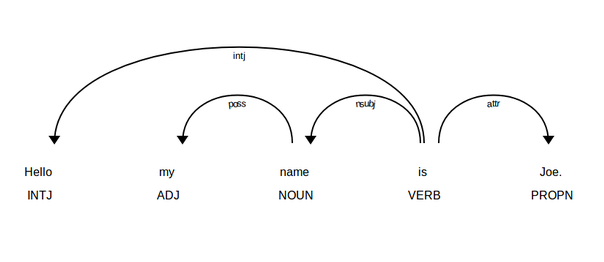
\includegraphics[width=.7\linewidth]{01.png}
		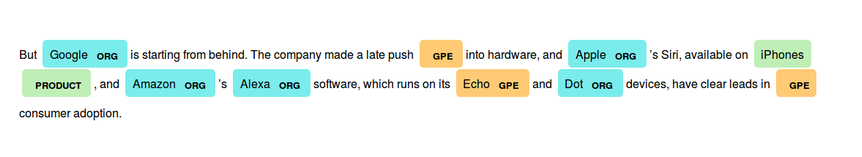
\includegraphics[width=.9\linewidth]{02.png}
		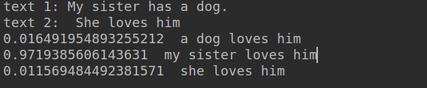
\includegraphics[width=.7\linewidth]{03.png}
	

\end{figure}

\end{frame}
%------------------------------------------------
\begin{frame}
\frametitle{Methodology}
\begin{itemize}
	\item \textcolor{gray}{Analysis  the  given  APD  symptoms  by  speech  
		recognition  based  on  Deep  learning}
	\item Analysis  the  given  APD  therapy  and  recommend  the
	
	treatment  to  the  APD  children.  Apply  a  natural  language
	
	processing  (NLP)  to  generate  sentences  and  exploit  Deep
	
	learning  to  understand  the  context  of  the  speech
	
	\item \textcolor{gray} {Monitoring  the  process  of  APD  treatment  by  using  speech 	 analysis  based  on  Deep learning}
	
\end{itemize}

\end{frame}

\begin{frame}
\frametitle{Techniques}
\textbf{Proposal for the objective 2 solution}
\begin{columns}	
\begin{column}{.5\textwidth}
	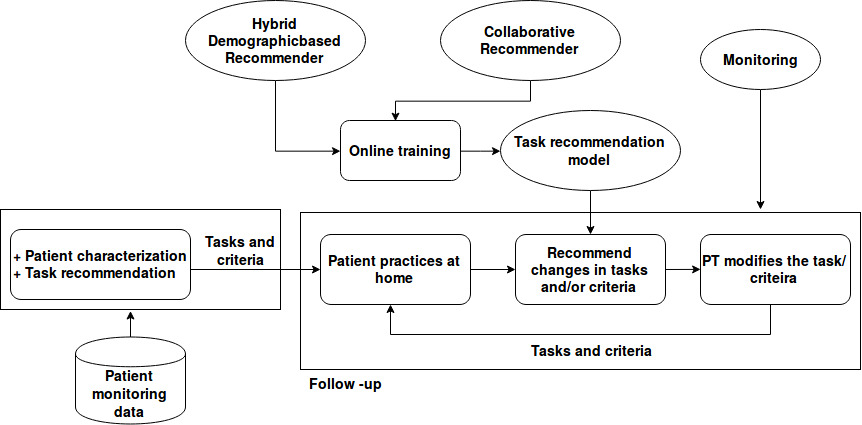
\includegraphics[width=65mm]{f3(1).jpg}
\end{column}
\begin{column}{.5\textwidth}
	
	\begin{itemize}
		\item Propose a training therapy to the APD kid based on the diagnosing report and Task recommendation model
		\item Monnitor the progress of therapy
		\item Update the monitoring data
		\item Suggest the fit training therapy by using reinforcement learning based on recommendation system
	\end{itemize}
	
\end{column}
\end{columns}
\end{frame}


\begin{frame}
\textbf{Task recommendation model \footnote{https://www.thebsa.org.uk}}
\begin{center}
	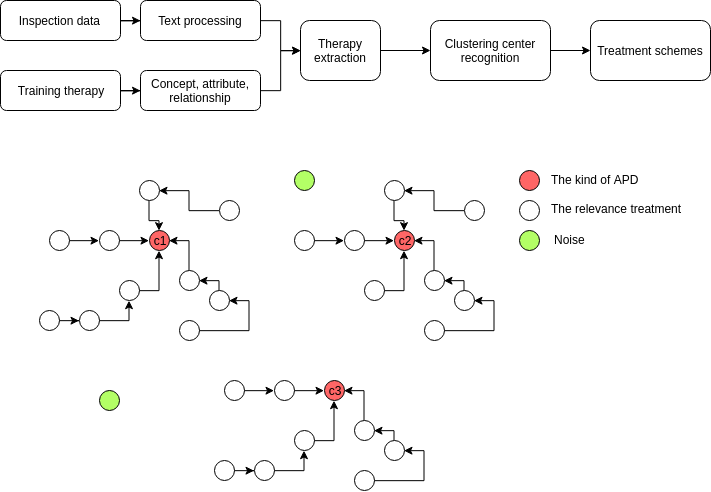
\includegraphics[width=100mm]{11.png}
\end{center}
\end{frame}

\begin{frame}
\textbf{Tasks and criteria}\\
\begin{columns}	
	\begin{column}{.5\textwidth}
		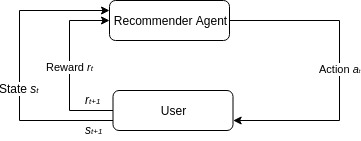
\includegraphics[width=65mm]{RL.jpg}
	\end{column}
	\begin{column}{.5\textwidth}
	\begin{itemize}
		\item State space $\mathcal{S}$: A state $s_t = \{s_t^i\}, i = (1,N)$
		\item  Action space $\mathcal{A}$: An action $a_t = \{a_t^j\}, j =( 1, K)$
		\item Reward $\mathcal{R}$: $r(s_t,a_t)$ according to the user's feedback
		\item Transition probability $\mathcal{P}$: $p(s_{t+1}|s_t,a_t)$ defines the probebility of state transition from $s_t$ to $s_{t+1}$ when Recommender Agent takes action $a_t$
	\end{itemize}
\end{column}
\end{columns}
\end{frame}



%------------------------------------------------
\begin{frame}
\frametitle{Methodology}
\begin{itemize}
\item \textcolor{gray}{Analysis  the  given  APD  symptoms  by  speech  
recognition  based  on  Deep  learning}
\item \textcolor{gray} {Analysis  the  given  APD  therapy  and  recommend  the 	treatment  to  the  APD  children.  Apply  a  natural  language 	processing  (NLP)  to  generate  sentences  and  exploit  Deep 	learning  to  understand  the  context  of  the  speech}

\item Monitoring  the  process  of  APD  treatment  by  using  speech analysis  based  on  Deep learning

\end{itemize}

\end{frame}
%------------------------------------------------


\begin{frame}
\frametitle{Techniques}
\textbf{Proposal for the objective 3 solution}\\


\begin{itemize}
\item Convert the APD speech to text
\item Analysis the meaning of the text
\item Make the score of the benchmark table

\item Make the client-server model to monitor and evaluate the progress of each patient
\end{itemize}


\end{frame}

\begin{frame}
\begin{figure}
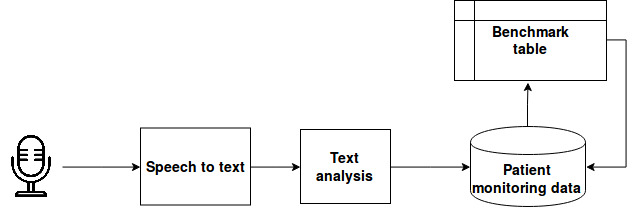
\includegraphics[width=65mm]{f4.jpg}
\end{figure}

Describe the score of the training for the respective user at home
\begin{table}[]
	\begin{tabular}{|l|l|l|l|l|}
		\hline
		\textbf{}                                                         & Observation & Assessment & \begin{tabular}[c]{@{}l@{}}Therapy \\ lesson\end{tabular} & Other \\ \hline
		Listening                                                         &             &            &                                                              &       \\ \hline
		Speaking                                                          &             &            &                                                              &       \\ \hline
		\begin{tabular}[c]{@{}l@{}}Phonological \\ Awareness\end{tabular} &             &            &                                                              &       \\ \hline
	\end{tabular}
	\caption{Benchmark table}
	\label{2}
\end{table}
\end{frame}

\begin{frame}
\frametitle{Client and Master MedicBot}
\begin{columns}	
	\begin{column}{.5\textwidth}
		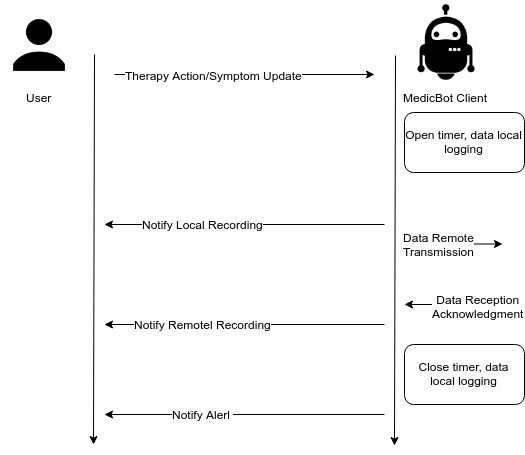
\includegraphics[width=55mm]{client.jpg}
	\end{column}
	\begin{column}{.5\textwidth}
		
			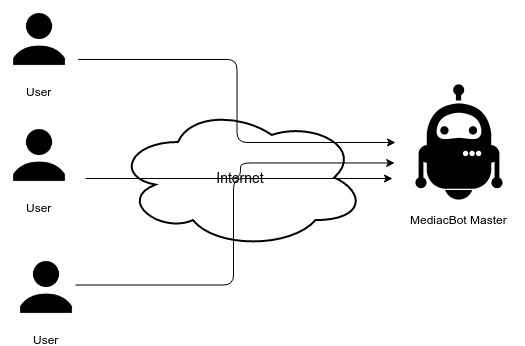
\includegraphics[width=55mm]{Master.jpg}
		
	\end{column}
\end{columns}
MedicBot Client collects data from User and then send them to the MedicBot Master to store and analysis more (if the problem needs specialists)
\end{frame}
\section{Conclusion}
\begin{frame}
\frametitle{Conclusion}

\begin{itemize}
	\item MedicBot is a new approach for building a Medical assistance for Auditory Processing Disorder (APD) children. 
	\item In this framework, the text analysis is of paramount importance and its strategy should be learned from data and adapted online, to address the possible evolution of the APD problem. 
	
	\item Many challenges remain to build a complete system based on this proposition such as: out-of-domain handling applications overestimating their scores, adaptation to a specific  user ,  non  stationary  usages  of  sets  of  application and more generally co-adaptation belong to our concerns. 
\end{itemize}
\end{frame}
\begin{frame}{}
\centering \Huge
\emph{Thank You}
\end{frame}
%------------------------------------------------



\end{document}